\section{OBS TCEs}

\begin{enumerate}
\item Summary of how this TCE population differed, especially compared to DR24 and Q1-Q16.
\item Basic stats of the distribution of TCEs in Period and maybe MES.
\item Describe what information comes from the pipeline.
\item There are way more TCEs than expected KOIs, the task at hand is to filter out the transit-like, astrophysical events and turn them into KOIs. Amongst those, identify which of those are likely planet candidates.  

\end{enumerate}

\label{tces}
As with the previous three Kepler planet candiate catalogs \citep{Coughlin2016cat,Mullally2015cat,Rowe2015cat}, the population of events that were used to create KOIs are known as Threshold Crossing Events or TCEs.  These are periodic dimmings of a light curve that were found by the  Transit Planet Search module and validated by the Data Validation module of the Kepler pipeline \citep{Jenkins2017kdph, Fanelli2011}.   The Data Release 25 TCEs were created by running the SOC 9.3 version of the pipeline on the Kepler data release 25, Q1--Q17 \Kepler\ PDC time-series.  For a thorough analysis of the DR25 TCEs and on the pipeline's search see \citet{Twicken2016}.  The DR25 TCEs, their ephemerides, and the metrics calculated by the pipeline are available at the NASA Exoplanet Archive \citet{Aekeson2013}.  In this paper we endeavor to disposition these signals into planet candidates and false positives.   Because the TCEs act as the input to our catalog, we first describe some of their properties as a whole and reflect on how they are different than the previous TCE table.

The DR25 TCE table at NExScI contain 34,032 DR25 OBS TCEs (Observed TCEs), however, in this paper we disposition 32,534 of these TCEs. The remaining TCEs are known as ``bogus" TCEs, and were created because of a bug in the Kepler pipeline. Because the primary purpose of this catalog is to be able to calculate occurrence rates and because this same bug was not present when characterizing the pipeline, we ignore the bogus TCEs here. For more information see the documentation for the occurence rate products \citet{Burke2017} 

We have plotted the distribution of the 32,534 TCEs in terms of both Period and MES (Multiple Event Statistic, a statistic that measures the significance of the event, see \citep{Jenkins2002a}), in Figure~\label{f:tces}. Notice an excessive number of short and long period TCEs, as well as many low MES TCEs.  

\begin{figure*}
 \begin{center}
  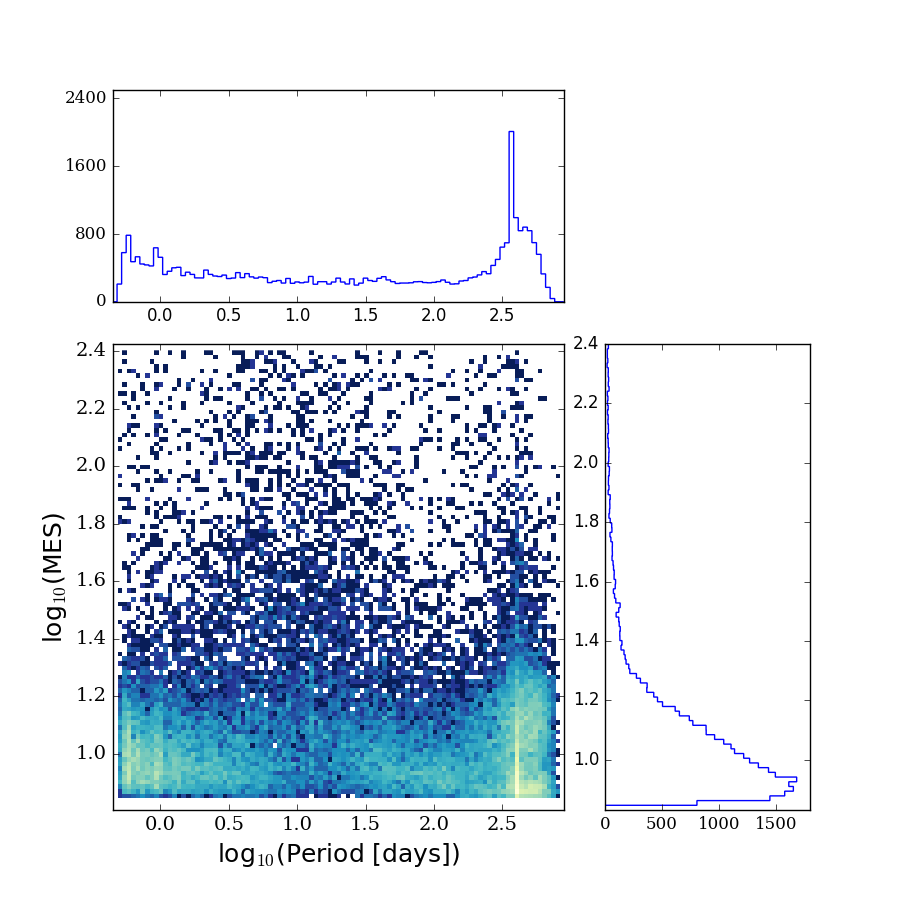
\includegraphics[width=\linewidth]{tce-dist.png}
  \caption{\ref{f:tces} A two dimensional histogram of the number of TCEs by log(period) and log(MES). The marginalized distributions for log(period) and log(MES) are projected along their respective axes and shown on the top and right respectively. }
 \end{center}

As with previous TCE catalogs, the short period ($\lt 10$\,d) excess is dominated by true, sinusoidal variability of the star. The long period excess is dominated by instrumental noise. A decrease in flux caused by a cosmic ray hit (a.k.a. SPSD, Sudden Pixel Sensitivity Drop-out), can match-up with natural fluxuations in the data to produce a TCE. Also image artifacts known as rolling-band is very strong on some channels \citep[see p??][]{KDCH} and since the spacecraft rolls every 90\,days, these variations can easily line-up to produce many TCEs at 370\,d.  This excess of long period TCEs is significantly larger than in the previous, DR24 TCE catalog \citep{Seader2015}. This is most likely because DR24 implemented an aggressive and irregular veto known as the bootstrap metric.  For DR25 this metric was calculated \citep{Jenkins2016}, but was not used as a veto.  Also other vetos were tuned down causing more TCEs across all periods to be created.

To summarize, for DR25 the number of false signals in the TCE table is drastically larger than in any previous catalog. This has two effects, the first is that it should allow through more true exoplanets, but it also reduced the reliability of a random TCE event. 


\end{figure*}
